\chapter{Desarrollo experimental}
	
	Este trabajo busca realizar una investigación cuasi-experimental para reportar el comportamiento  del destilador solar propuesto de acuerdo a la influencia de las variables independientes descritas en la~\cref{table:variables-independientes-desarrollo-experimental}.
	
	\begin{longtblr}[
		caption = {Variables del desarrollo experimental},
		label = {table:variables-independientes-desarrollo-experimental},
		note{*} = {Se puede ejercer control directo sobre esta variable.}
	]{
		colspec = {X[l] c c X[2, l]},
		hlines,
		vlines,
		row{odd} = {bg=tablerowblue},
		row{1} = {
			bg = tabletitleblue,
			fg=white,
			font = \bfseries,
			halign=c
		},
		rowhead = 1,
		rows={m}
	}
		Variable & Clasificación & Tipo de dato & Influencia en el modelo\\
		Temperatura de entrada del agua\TblrNote{*}
			& Independiente
			& Cuantitativa
			& Establece la temperatura inicial del modelo térmico para la ebullición del agua\\
		Presión atmosférica
			& Independiente
			& Cuantitativa
			& Modifica la temperatura a la cual sucede el cambio de fase del agua\\
		Temperatura ambiente
			& Independiente
			& Cuantitativa
			& Influye en las pérdidas de calor que tendrá el sistema\\
		Clima (nubosidad)
			& Independiente
			& Cualitativa
			& Punto de comparación rápido para ver la influencia de la nubosidad sobre el desempeño\\
		Velocidad de viento
			& Independiente
			& Cuantitativa
			& Se asocia directamente a las pérdidas de calor por convección\\
		Hola del día
			& Independiente
			& Cuantitativa
			& Determina la posición angular del Sol y se relaciona con la irradiación solar\\
		Irradiación solar promedio
			& Independiente
			& Cuantitativa
			& Determina la potencia solar recibida en nuestro modelo de transferencia de calor\\
		Temperatura de salida del agua
			& Dependiente
			& Cuantitativa
			& Asociada al cambio de fase del agua\\
		Temperatura del recibidor solar
			& Dependiente
			& Cuantitativa
			& Influye en los modelos térmicos para la destilación del agua\\
		Caudal de agua\TblrNote{*} 
			& Dependiente
			& Cuantitativa
			& Influye en los modelos térmicos y la tasa de desalinización\\
		Propiedades físico-químicas del agua
			& Dependiente
			& Cuantitativa
			& Indica la calidad del agua
	\end{longtblr}
	
	\section{Grupos de estudio}
		
		Con base en las variables observadas en la~\cref{table:variables-independientes-desarrollo-experimental} se distinguieron los grupos de control descritos en las sub-secciones siguientes.
		
		\subsection{Agua}
			
			Las muestras de agua se seleccionaron guiándose en la~\cref{table:clasificacion-agua-tds}. Para ello, la obtención de agua de mar se simula con sales marinas para acuario y se proponen 3 grupos de control descritos en la~\cref{table:grupo-control-agua} para evaluar los casos límite y promedio de la salinidad del agua de mar.
			
			\begin{longtblr}[
				caption = {Grupo de control del agua de mar},
				label = {table:grupo-control-agua}
			]{
				colspec = {X[c] X[2, c]},
				hlines,
				vlines,
				width = 0.5\linewidth,
				rowhead = 1,
				row{odd} = {bg=tablerowblue},
				row{1} = {
					bg = tabletitleblue,
					fg=white,
					font = \bfseries,
					halign=c
				},
				rows={m}
			}
				Muestra & Salinidad (\unit{\mg\per\litre})\\
				1 & \num{30000}\\
				2 & \num{35000}\\
				3 & \num{40000}
			\end{longtblr}
		
		\subsection{Lugar físico de experimentación}\label{sec:ch6-lugar-fisico}
			
			Debido al alcance del proyecto, se acotó el lugar físico de experimentación a la Unidad Profesional Interdisciplinaria en Ingeniería y Tecnologías Avanzadas ubicada en la Ciudad de México.
			
			\begin{longtblr}[
				caption = {Grupo de control del agua de mar},
				label = {table:grupo-control-fisico}
			]{
				colspec = {X[c] *{3}{c}},
				hlines,
				vlines,
				width = 0.8\linewidth,
				rowhead = 1,
				row{odd} = {bg=tablerowblue},
				row{1} = {
					bg = tabletitleblue,
					fg=white,
					font = \bfseries,
					halign=c
				},
				rows={m}
			}
				Zona & Longitud & Latitud & Altitud\\
				Ciudad de México, México
					& \ang{-99;07;32}
					& \ang{19;30;38}
					& \qty{2241}{\m}
			\end{longtblr}
			
			\subsubsection{Variables climáticas sobre la región a investigar}
				
				Debido a la naturaleza de nuestra fuente de energía y que su operación no transcurren dentro de un ambiente controlado se deben evaluar las condiciones climáticas del lugar que impactan en mayor medida el sistema propuesto.
				
				\begin{longtblr}[
					caption = {Variables climáticas consideradas importantes para la investigación},
					label = {table:variables-climaticas},
					note{?} = {Se decidió incluir en el estudio a esta variable dado a que no se sabe con certeza si será necesaria para el futuro desarrollo.}
				]{
					colspec = {X[c] X[3, l] c},
					hlines,
					vlines,
					width = \linewidth,
					row{odd} = {bg=tablerowblue},
					rowhead = 1,
					row{1} = {
						bg = tabletitleblue,
						fg=white,
						font = \bfseries,
						halign=c
					},
					rows={m}
				}
					Variable & Descripción & Unidades\\
					Presión superficial
						& Presión promedio en la superficie del lugar
						& \unit{\kilo\pascal}\\
					Velocidad de viento
						& Velocidad de viento promedio a 2 metros sobre la superficie del lugar
						& \unit{\m\per\s}\\
					Humedad específica
						& Razón promedio de la masa de vapor de agua por unidad de aire a 2 metros sobre la superficie del lugar
						& \unit{\gram\per\kg}\\
					\acrfull{roc} sobre cielo despejado
						& Total de irradiación solar incidida (directa más difusa) sobre la tierra en un plano horizontal sobre la superficie de la tierra a condiciones de cielo despejado.
						& \unit{\watt\hour\per\m\tothe{2}}\\
					\acrlong{roc}
						& Total de irradiación solar incidida (directa más difusa) sobre la tierra en un plano horizontal sobre la superficie de la tierra a todas las condiciones.
						& \unit{\watt\hour\per\m\tothe{2}}\\
					Nubosidad
						& Porcentaje promedio de cantidad de nubes en el cielo sobre un lapso determinado
						& \unit{\watt\hour\per\m\tothe{2}}\\
					Irradiancia UVA\TblrNote{?}
						& Radiación UVA (\qtyrange{315}{400}{\nm}) total incidida a todas las condiciones climáticas del día
						& \unit{\watt\per\m\tothe{2}}\\
					Irradiancia UVB\TblrNote{?}
						& Radiación UVB (\qtyrange{280}{315}{\nm}) total incidida a todas las condiciones climáticas del día
						& \unit{\watt\per\m\tothe{2}}	
				\end{longtblr}

	\section{Selección y caracterización del elemento óptico de concentración}
		
		Para este proyecto son accesibles 4 modelos de lentes de Fresnel con ranuras hacia adentro cuyas características se ven resumidas en la~\cref{table:fresnel-lenses-models}.
		
		% Página 36
		\begin{longtblr}[
			caption = {Modelos y características de los concentradores solares},
			label = {table:fresnel-lenses-models}
		]{
			colspec = {*{2}{X[1.5]} *{2}{X} X[2.5] *{2}{X}},
			hlines,
			vlines,
			width = \linewidth,
			rowhead = 2,
			row{odd[3]} = {bg=tablerowblue},
			row{1,2} = {
				bg = tabletitleblue,
				fg=white,
				font = \bfseries,
				halign=c
			},
			rows={
				halign = c,
				valign = m
			}
		}
			Modelo & Longitud focal & Ancho & Largo & Material & Grosor & Tamaño de ranura\\
			--- & mm & mm & mm & --- & mm & mm\\
			CP220-280
				& \num{220}
				& \num{280}
				& \num{280}
				& PMMA: \acrshort{pvuvc}
				& \num{5}
				& \num{0.5}\\
			CP330-280
				& \num{330}
				& \num{280}
				& \num{280}
				& PMMA: \acrshort{pvuvc}
				& \num{5}
				& \num{0.5}\\
			CP350-300 
				& \num{350}
				& \num{310}
				& \num{310}
				& PMMA: \acrshort{pvuvc}
				& \num{5}
				& \num{0.5}\\
			CP350-330 
				& \num{350}
				& \num{340}
				& \num{340}
				& PMMA: \acrshort{pvuvc}
				& \num{5}
				& \num{0.5}
		\end{longtblr}
		
		Se halla en su hoja técnica que el PMMA \acrshort{pvuvc} tiene una transmitancia igual a \percent{92.65}.
		
		Para seleccionar la lente se tomó como criterio principal el número F (\gls{F}) dado por \eqref{equ:F-number}, ya que entre mayor sea \gls{F}, será mayor la capacidad de concentración y será mejor la capacidad de recolección de la lente.
		
		\begin{equation}\label{equ:F-number}
			\gls{F} = \dfrac{\gls{f}}{2\gls{Rl}}
		\end{equation}
		
		Conociendo eso, se determina que el modelo a usar es la lente de Fresnel condensadora \textbf{CP330-280} con un \gls{F} equivalente a \num{1.179}. 
		
		A continuación se enlistan algunas propiedades importantes del material seleccionado \cite{shannon_art_1997} citado por \cite{leutz_nonimaging_2001}.
		
		\begin{itemize}
			\item Índice de refracción: $\gls{nd} = 1.4918$
			\item Número de Abbe: $V_d = 54.7$
			\item Coeficiente de temperatura: $\sfrac{dn}{dT} \unit{\per\kelvin} = \num{-105e-6}$
		\end{itemize}
		
		Conociendo esto se calculan los ángulos $\alpha$, $\omega$ y $\beta$ necesarios para el cálculo en el trazado de rayos usando \cref{equ:rayos-alfa,equ:rayos-omega,equ:rayos-beta}. Donde $\alpha$ es la inclinación del prisma y $\beta$ es el ángulo del prisma.
		
		\begin{align}
			\tan\alpha &= \dfrac{R}{\gls{nd}\sqrt{R^{2}+f^{2}} - f} \label{equ:rayos-alfa}\\
			\tan\omega &= \dfrac{R}{f} \label{equ:rayos-omega}\\
			\tan\beta &= \alpha + \omega \label{equ:rayos-beta}
		\end{align}
		
		Lo que nos da: $\alpha= \ang{34.361}$, $\omega = \ang{22.989}$, $\beta= \ang{57.350}$
		
		Finalmente se describen las ecuaciones que se usan para modelar el trazado de rayos.
		
		\begin{align}
			\phi_{1} &= \beta - \alpha - \theta_{\text{entrada}}\\
			\phi_{1}\prime &= \arcsin\left(\dfrac{\sin\phi_{1}}{\gls{nd}\prime}\right)\\
			\phi_{t} &= \beta - \alpha - \phi_{1}\prime\\
			\phi_{2}\prime &= \phi_{t} + \alpha\\
			\phi_{2} &= \arcsin{\sin\phi_{2}\prime\gls{nd}\prime}\\
			\theta_{salida} &= \phi_{2} - \alpha
		\end{align}
		
		
	
	\section{Diseño de la cámara de concentración solar}
		
		\subsection{Recibidor solar}
			
			Para el recibidor solar se comparó (\cref{table:comparacion-material-recibidor}) la propuesta de dos materiales típicamente usados para la manufactura de recibidores solares.
									
			\begin{longtblr}[
				caption = {Comparativa hallada entre los materiales propuestos para fungir como recibidor solar},
				label = {table:comparacion-material-recibidor},
			]{
				colspec = {l c *{2}{X[c]}},
				hlines,
				vlines,
				row{odd} = {bg=tablerowblue},
				row{1} = {
					bg = tabletitleblue,
					fg=white,
					font = \bfseries,
					halign=c
				},
				rowhead = 1,
				rows={m}
			}
				Propiedad & Unidades & Cobre & Carburo de Silicio\\
				Conductividad térmica 
					& \unit{\watt\per\m\kelvin}
					& \numrange{387.0}{430.0}% \cite{leonel_lira_cortes_conductividad_2010}
					& \numrange{120}{130}\\ % https://www.gab-neumann.com/Carburo-de-silicio-Propiedades https://geologiaweb.com/materiales/carburo-de-silicio/
				Coficiente de expansión térmica 
					& \unit{\per\degreeCelsius}
					& \num{16.5e-6}
					& \num{4e-6}\\
				Densidad
					& \unit{\kg\per\m\tothe{3}}
					& 8620
					& 3210\\
				Resistencia a la corrosión
					& ---
					& Menor
					& Mayor\\
				Costo
					& MXN
					& Menor
					& Mayor\\
				Accesibilidad
					& ---
					& Mayor
					& Menor\\
				Propiedades ópticas
					& ---
					& Alta reflectividad de luz en el espectro visible
					& Se puede manufacturar para tener buena absortividad
			\end{longtblr}
			
			Con base en la comparativa anterior, se decide el uso de cobre como material para el recibidor solar. Para mejorar sus características como recibidor solar se aplicará un recubrimiento que potencie sus características usando el principio de selectividad espectral. 
			
			Se considera que el recubrimiento de óxido negro resulta ser una opción adecuada ya que de acuerdo al resultado reportado en \cite{lowery_solar_1977}, alcanza valores de absortividad para el espectro solar en el rango de 0.78 a 0.86 y de emisividad de 0.04 a 0.08.
%			
%			\begin{itemize}
%				\item Se prepara una disolución de sales de ``ebolnol C'' en agua a una concentración de \qty{180}{\gram\per\litre}
%				\item Se calienta la disolución a las instrucciones dadas por el fabricante o en su defecto a \qty{372}{\kelvin}.
%				\item Se sumerge el área de interés sobre la 
%			\end{itemize}
			
		\subsection{Almacenamiento térmico de calor}
			
			Como se ha resaltado a lo largo del texto, el sol es una fuente intermitente de energía, por lo que se propone un mecanismo de almacenamiento térmico de calor empleando arena de sílice de alta pureza la cual es una arena compuesta mayormente por \ch{SiO2}. Las propiedades más relevantes encontradas en \cite{davenport_thermal_2022} y \cite{wypych_2_2021} y por las que se decidió por este material se enumeran a continuación.
			
			\begin{itemize}
				\item \textbf{Excelente estabilidad térmica}: Se habla que la arena de sílice de cuarzo-$\alpha$ es estable hasta los \qty{573}{\degreeCelsius} donde sufre solamente una alteración de los ángulos en las uniones de la red cristalina para transformarse en cuarzo-$\beta$. Esta transformación es rápidamente reversible y no involucra ningún rompimiento de enlaces.
				\item \textbf{Alta capacidad calorífica}: En el estudio se observó que de temperatura ambiente hasta los \qty{1200}{\degreeCelsius} presenta una capacidad calorífica de \qtyrange{750}{1200}{\joule\per\kg\kelvin}
				\item \textbf{Conductividad térmica adecuada:} Gracias a que su conductividad no es demasiado alta ni demasiado baja (\qtyrange{7.2}{13.6}{\watt\per\m\kelvin}) no representa un problema hablando de pérdidas de calor.
				\item \textbf{Coeficiente de expansión térmica:} Posee un coeficiente de expansión térmica linear igual a \qty{14e-6}{\per\kelvin}.
				\item \textbf{Densidad}: \qty{2.65}{\g\per\cm\tothe{3}}
				\item \textbf{Humedad}: Aproximadamente \percent{0.1}
			\end{itemize}
			
%		\subsection{Aislamiento térmico}
%			
%			Se realizó una investigación previa sobre loa materiales candidatos como aislantes térmicos de los cuales se determinó que los siguientes materiales son potenciales candidatos: aereogel, fibra de sílice, fibra cerámica.
			
		\subsection{Pérdidas}
			
			\subsubsection{Pérdidas por transmisión}
				
				Usando como referencia la~\cref{fig:Transmitancia} vemos que el elemento de concentración tiene una eficiencia de transmisión aproximada de \percent{85}. Además el cuarzo utilizado como ventana en la cámara tiene una eficiencia de transmisión de \percent{90.89}, asumiendo que el aire es un medio con $\gls{nd}_{\text{aire}} = 1$ y $\gls{tau}_{\text{aire}} = 1$, la transmisión total del sistema estaría dada por \eqref{equ:transmisión-cámara}.
		
				\begin{figure}[H]
					\centering
					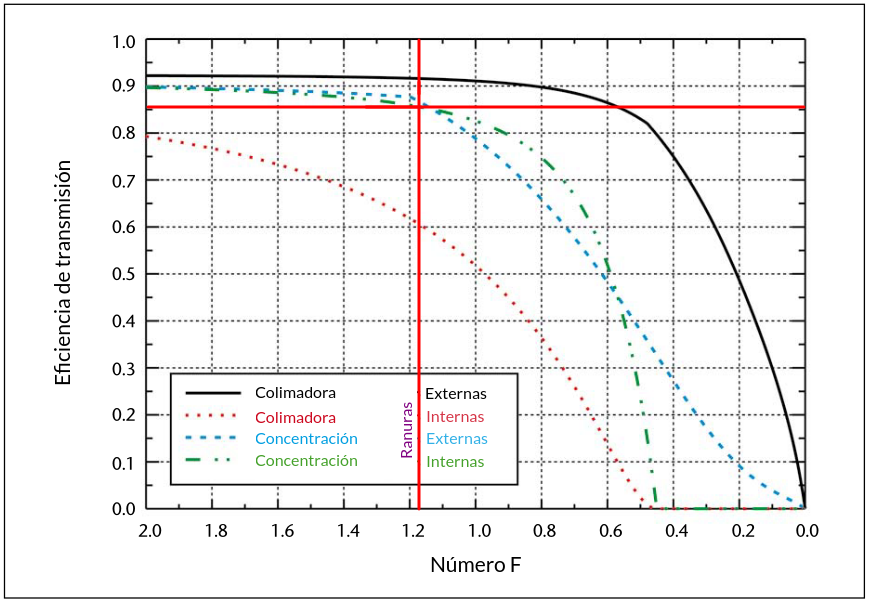
\includegraphics[
						width=\linewidth,
						height=70mm,
						keepaspectratio
					]{Desarrollo-experimental/Transmitancia.png}
					\caption{Valores de eficiencia idealizados de lentes de Fresnel calculadas en la reflexión de las superficies y otras pérdidas comunes.}
					\floatfoot{Imagen adaptada de \cite{davis_optical_2007}}
					\label{fig:Transmitancia}
				\end{figure}
				
				\begin{equation}\label{equ:transmisión-cámara}
					\gls{tau} = \tau_{\text{lente}}\tau_{\text{cuarzo}} = \percent{77.26}
				\end{equation}